\documentclass{beamer}
\usetheme{Boadilla}
\usepackage[utf8]{inputenc}
\usepackage[czech]{babel}
\usepackage{hyperref}
\usepackage{listings}
\usepackage{graphicx}
\usepackage{wrapfig}
\usepackage{epsfig}
\usepackage{multicol}

\title{IoT Akvárium}
\author{Martin Beránek}
\lstset{language=C++,
        basicstyle=\ttfamily\scriptsize,
        keywordstyle=\color{blue}\ttfamily,
        stringstyle=\color{red}\ttfamily,
        commentstyle=\color{green}\ttfamily,
        breaklines=true,
		float=h
}

\begin{document}
	\frame{\titlepage}
	\section{Návrh}
	\begin{frame}{Úvod}
		Automatizovat akvárium co nejlevněji.
		\begin{itemize}
			\item Email notifikace,
			\item Měření:
			\begin{itemize}
				\item Hladina,
				\item Teplota.
			\end{itemize}
			\item Spínání:
			\begin{itemize}
				\item Filtru,
				\item Světla,
				\item Zahřívání vody.
			\end{itemize}
			\item Krmení!
		\end{itemize}
	\end{frame}
	\begin{frame}{Součástky}
		\begin{itemize}
			\item Krokový motor,
			\item Teploměr,
			\item Spínací plovák,
			\item Arduino + Ethernet Shield,
			\item Relé,
			\item a bohužel také RTC.   			
		\end{itemize}
	\end{frame}
	\begin{frame}{Schema}
		\begin{center}
			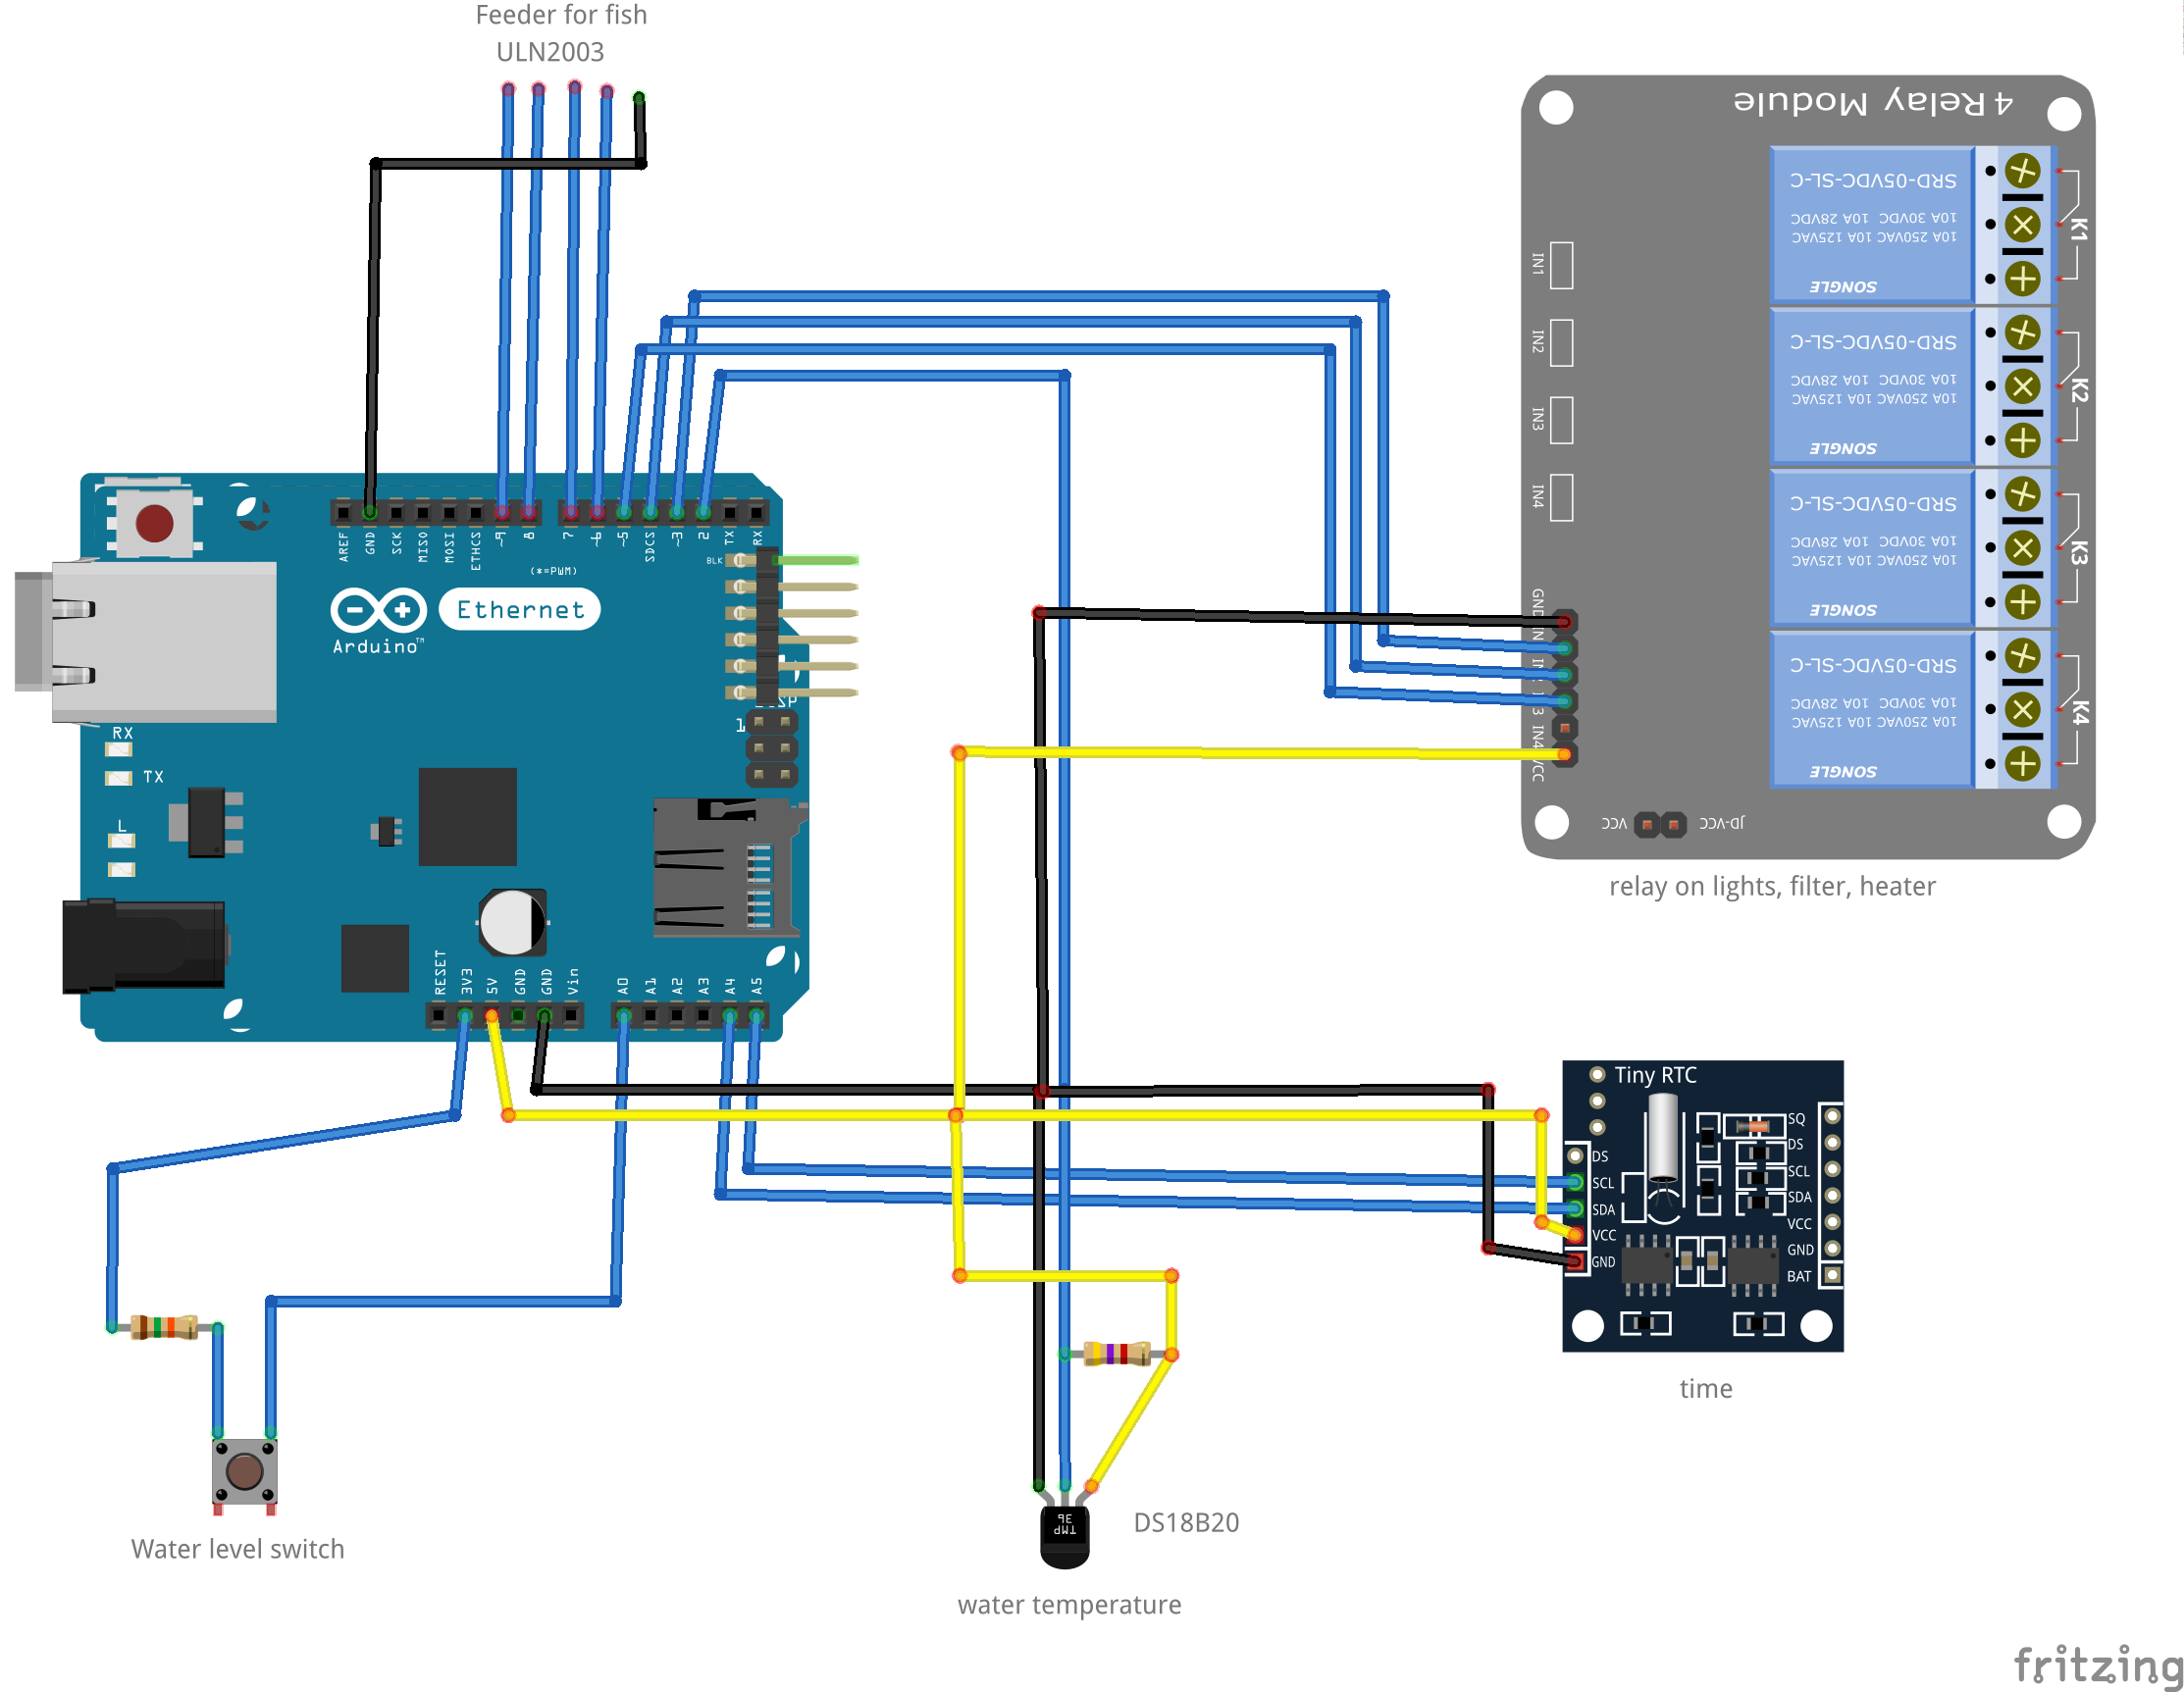
\includegraphics[scale=0.4]{schema_bb.png}
		\end{center}
	\end{frame}
	\begin{frame}{Zapojení}
		\begin{itemize}
			\item Arduino připojené přes Ethernet,
			\item Server sbírá data do databáze,
			\item Cacti vykresluje grafy,
			\item Klient si může prohlédnout grafy ve webovém výstupu Cacti.	
		\end{itemize}
	\end{frame}
	\begin{frame}{Připojení}
		\begin{center}
			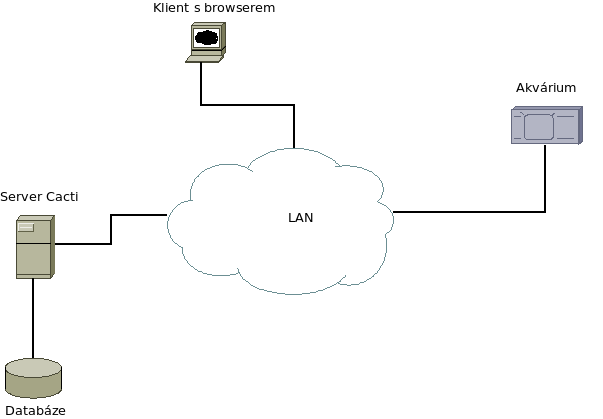
\includegraphics[scale=0.4]{net.png}
		\end{center}
	\end{frame}
	\begin{frame}{Cacti}
		\begin{center}
			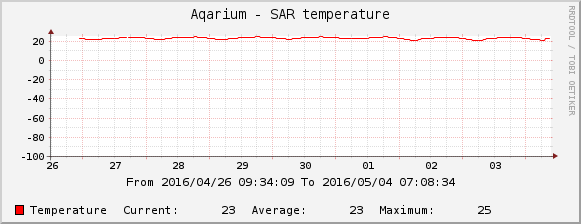
\includegraphics[scale=0.5]{graph.png}
		\end{center}
	\end{frame}
\end{document}
